% $Id

%% Dokumentenklasse (Koma Script) -----------------------------------------
\documentclass[%
   %draft,     % Entwurfsstadium
   final,      % fertiges Dokument
	 % --- Paper Settings ---
   paper=a4,% [Todo: add alternatives]
   paper=portrait, % landscape
   pagesize=auto, % driver
   twocolumn,
   % --- Base Font Size ---
   fontsize=10pt,%
	 % --- Koma Script Version ---
   version=last, %
 ]{scrartcl} % Classes: scrartcl, scrreprt, scrbook


% Encoding der Dateien (sonst funktionieren Umlaute nicht)
% Fuer Linux -> utf8
% Fuer Windows, alte Linux Distributionen -> latin1

% Empfohlen latin1, da einige Pakete mit utf8 Zeichen nicht
% funktionieren, z.B: listings, soul.

%\usepackage[latin1]{inputenc}
%\usepackage[ansinew]{inputenc}
\usepackage[utf8]{inputenc}
%\usepackage{ucs}
%\usepackage[utf8x]{inputenc}

\usepackage[T1]{fontenc}
\usepackage[english]{babel}

\addto\captionsenglish{
  \renewcommand{\contentsname}{Table of Contents}
}

\usepackage{multicol}
%\usepackage[scaled]{uarial}


\renewcommand{\rmdefault}{phv} % Arial
\renewcommand{\sfdefault}{phv} % Arial

\usepackage{appendix}
\usepackage{listings}
\usepackage{color}
\usepackage{geometry}
\usepackage{array}
\usepackage{graphicx}
\usepackage{caption}


\usepackage{subcaption}
%prefer subcaption instead of subfigure
%\usepackage{subfigure}

\usepackage{float}
%\usepackage{tikz}
%\usetikzlibrary{arrows}

\usepackage{tikz}
\usetikzlibrary{matrix,calc,shapes}

\tikzset{
  treenode/.style = {shape=rectangle, rounded corners,
                     draw, anchor=center,
                     text width=5em, align=center,
                     top color=white, bottom color=blue!20,
                     inner sep=1ex},
  decision/.style = {treenode, diamond, inner sep=0pt},
  root/.style     = {treenode, font=\Large, bottom color=green!30, align=center},
  env/.style      = {treenode, font=\ttfamily\normalsize},
  finish/.style   = {root, bottom color=green!40},
  dummy/.style    = {circle,draw}
}
\newcommand{\yes}{edge node [above] {yes}}
\newcommand{\no}{edge  node [left]  {no}}

%\usepackage{hyperref}

\sffamily

%% Titel -----------------------------------------
\title{Recognition of Human Facial Expressions by Mid-Level Discriminative Patches}
\subtitle{Research Project Master Artificial Intelligence Group 4}
\author{Stefan Selzer I6123079\\Chang Sun I6113630\\Ioannis Papadopoulos i6055779\\Salil Bhat}


%% Dokument -----------------------------------------
\begin{document}

%\begin{@twocolumnfalse}
\onecolumn

\maketitle
\thispagestyle{empty}

\newpage


\begin{abstract}

TODO: same as introduction, change one of them !!
\\
\\
Unsupervised Discovery of mid-level discriminative patches is a method to extract the primitives for visual information from an image.  Singh et al. elaborated on this method by stating that the primitives have to satisfy the requirements of being representative as well as discriminative and having been discovered in a fully unsupervised manner \cite{Singh2012DiscPat}. The method combines techniques from the fields of computer vision and machine learning to produce promising results in image recognition and classification. 
\\
\\
The aim of this project is to apply this method on the classification of images of human facial expressions. This can, for example, aid in human-computer interaction by recognizing particular emotions or cognitive states through visual or expressive features contained in an image. Then computers are enabled to react and interact with the counterpart in an appropriate manner. As a result of the project's work an application has been developed for classification of human emotions and the effectiveness of the image recognition by this classification will be proven with selected, distinct features of various images showing different facial expressions.
\end{abstract}

\thispagestyle{empty}

\newpage
\pagenumbering{roman}
\tableofcontents

\newpage
\listoffigures
\addcontentsline{toc}{section}{List of Figures}
\listoftables
\addcontentsline{toc}{section}{List of Tables}

\newpage
\pagenumbering{arabic}

%\end{@twocolumnfalse}

%\begin{multicols}{2}

\twocolumn



\section{Introduction}\label{sec:Introduction}
Unsupervised Discovery of mid-level discriminative patches is a method to extract from an image the primitives for visual information that satisfy the requirements of being representative as well as discriminative and that have been discovered in a fully unsupervised manner. The method was elaborated by Singh et Al. at the Carnegie Mellon University of Pittsburgh, Pennsylvania, and published at the European Conference on Computer Vision in the year 2012.\cite{Singh2012DiscPat} The method is settled in the fields of computer vision and machine learning and combines techniques from these fields to produce promising results in image recognition and classification. Singh et Al. showed the capabilities of their method in a follow-up publication What Makes Paris Look like Paris?.\cite{doersch2012what} Here they identified the most distinct elements on images of architecturally different cities like Paris and London classifying these images as being shot in the corresponding city.
\\
\\
The idea of this project is to apply this method on the classification of images of human facial expressions. This could for example aid in human computer interaction to recognize particular emotions or cognitive states through visual or expressive features contained in an image.
\\
Put in one phrase the goal of this project is to find classifiers for human facial expressions.
In detail the requirements are to deliver an extensible, easy-to use and well documented code base using C++ as programming language and the image processing library OpenCV as toolset for the basic techniques and algorithms needed to implement the functionality.
\\
\\
This paper describes the results of the research project by first giving an overview of the technical background and describing the method implemented by Singh et Al.. Then the project work is presented and finally and outlook on possible future work is given.

\section{Technological Background}\label{sec:StateArt}

This chapter gives an explanation of definitions used and an overview of the algorithm proposed by Singh et Al. as well as the image processing techniques used therein.

\subsection{Image Patches}

To explain the notion of mid-level discriminative patches it is best to first take a look at the different levels of visual information that can be retrieved from an image. Approaching from bottom-up, the lowest level would correspond to a single pixel. But single pixels do obviously not provide much useful information to describe features of the real world. From top-down, the highest level would be the image as a whole. This imposes several problems such as a high number of spatial configurations needed to describe objects as well as too much unnecessary information to describe certain features contained in that image. The best way is found in between by looking at parts of the image that are just right to describe a certain feature of an image. Such parts are called mid-level image patches.
\\
\\
Singh et Al. define such patches as being discriminative if they are representative concerning the described feature and different enough from other patches describing the same or any other feature. Additionally they require such patches to be detectable with "`high recall and precision"' in a large number of images.\cite{Singh2012DiscPat}

\subsection{Applied Techniques}

The algorithm to detect discriminative patches in an unsupervised manner mainly consists of three parts:
\\
The first one is to extract features from an image, then these features are clustered and the clusters are train a linear support vector machine (SVM) used to classify new elements in the end.
\\
\\
The feature extraction is supposed to be done using histogram of oriented gradients (HOG). The features are computed as intensity gradients for small parts of an image. The edge directions defined like this are then counted and concatenated to form a comprehensive descriptor. One of the key advantages of this technique is that it is invariant to geometric or photometric transformations.\cite{Dalal:2005:HOG:1068507.1069007}
\\
\\
Clustering is done using k-means clustering. K-means clustering partitions a dataset into a given number of clusters in such a way that the sum of the quadratic deviations from each cluster centroid is minimized. As metric usually the Euclidian distance is used.\cite{DBLP:series/lncs/CoatesN12}
\\
\\
A linear SVM separates points with a hyperplane that has a maximized distance to the nearest data points on each side of the plane. This can be used as binary classifier to classify input data according to recognized patterns. These patterns are obtained by training the SVM on positive and negative samples of data describing the problem that needs to be solved by classification.\cite{Chang:2011:LLS:1961189.1961199}

\subsection{Proposed Algorithm}

Applying these techniques, the feature extraction using HOG descriptors produces a large number of possibly overlapping patches at multiple scales. If one would now know that some of these patches are similar, these could be used to train a SVM for classification. Fortunately a similarity can also be produced by clustering the patches using k-means clustering. The problem with the low-level metric used by k-means clustering is that it does not produce good results on image patches. To address this again a SVM could be trained to produce a similarity metric needed to refine these clusters. So the clustering depends on the similarity metric of the SVM while the SVM itself depends on the clusters to be trained. To solve this problem the described approach is done in an iterative way. First the data is clustered in HOG space then a SVM is trained using the clusters to produce a metric which then is used to refine the clusters. This is done until a convergence criterion is reached. The final classifiers then are ranked according to their purity and discriminativeness.
\\
Purity is defined as the sum of the classifiers detection scores of the top cluster members.
\\
Discriminativeness describes the ratio of detections on the positive training data and the union of the positive and negative training data. This ratio should be low but still above 0.
\\
\\
The drawback of the described process is that classifier might suffer from overfitting. Overfitting occurs for example when the number of features exceeds the number of training datasets. The effect then is that the classifier does not predict by generalizing from what he has learned but memorizes input patterns and recalls them. It can be measured when the prediction of training samples is far more accurate than the prediction of unknown validation data. To prevent this overfitting Singh et Al. divided the input data of the algorithm consisting of positive examples containing the features that are searched and negative ones not containing this feature further into two datasets each. From these two positive and negative training datasets one will then act as training and the other one as validation dataset. In each iteration of the algorithm, the datasets are flipped for the next iteration to enhance the clusters by new feature patches. Furthermore, the best patches recognized in the validation dataset will be added to the training data patches to ensure even more diversity.\cite{Singh2012DiscPat}



\section{Developed Application for Image Classification}\label{sec:application}

This section presents the application that has been developed. The application can be used to train an SVM for each category of a catalog of images or predict images using already trained SVMs. For training, it loads a set of images and trains SVMs for the given categories. The classifiers work on the HOG features extracted from the input images. The steps of the algorithm that performs the image classification are described in a general manner. Details of the implementation can be found in the appendix section \ref{sec:devdoc}.
\\
\\
To train classifiers, the application loads a catalog of images from the file system. At least 2 different categories have to be provided in separate sub folders. The folder names denote the category labels. If it is desired to obtain more data samples to enhance the training of the classifiers, additional images from the horizontally flipped versions of the input images are computed and added to the input data. This doubles the original sample size and eases the problem of overfitting. To improve the quality of the images in regard of the performed feature extraction, histogram equalization is applied to the images as a preprocessing step of the feature extraction. This increases the contrast of the images and produces sharper edges for the edge gradient computation of the feature extractor. The feature extraction is performed using Histogram of Oriented Gradients. The computed features are split into defined parts for training and validation purpose. If there are multiple samples from a similar source contained in the dataset, the separation will make sure that they are not distributed across the training and validation data. For each category, a training and a validation matrix is built each by the corresponding elements of the category itself as positive samples and an equal number of evenly distributed samples from all other corresponding categories as negative samples. The training matrix is used to train a classifier for each category. The validation matrix is used to test and validate the effectiveness of the trained classifier with a large number of unknown samples. Cross validation can be performed by exchanging the training and the validation matrix to enhance the SVMs with additional data. Finally the trained classifiers can be saved to disc for further usage. There will be one classifier for each category.

\section{Training Data}

%TODO: describe setup of datasets sued for training and validation.Present results

For training a system to recognize facial expression effectively, the dataset should focus on several main expressions namely anger, disgust, fear, happiness, sadness and surprise. Moreover, to ensure diversity in training, a proper dataset should be composed of faces with kinds of face shapes, colors, facial and scalp hairs from many participants with different genders, ethnic backgrounds and ages.


\subsection{Cohn-Kanade Facial Expression Dataset}
\nocite{Kanade2000CK+}\nocite{Lucey2010CK+}

The dataset used in this project was adopted from the Cohn-Kanade Facial Expression Database. The dataset refers to the emotions anger, contempt, disgust, fear, happiness, sadness, surprise and neutral. There are 5105 images from 123 subjects, with ages ranging from 18 to 30 years. Sixty-five percent of subjects were female, eight-five percent were Euro-American and fifteen percent were African-American and Asian. They were photographed in same temporal settings and were aligned directly in front of camera. Therefore all images have uniform background and lighting. The images were digitized into 640*480 or 490 pixel arrays with 8-bit precision for grayscale values and are available in png and jpg format.
\\
\\
In the Cohn-Kanade Facial Expression Dataset, subjects performed a series of several facial displays that varied from mild to intense expression for each emotion and images were taken frame by frame.  In the mild ones, the emotion is barely noticeable and in the intense ones, it is clearly noticeable. In order to train a robust system, we chose the images mostly with intense expressions which were clearly noticeable. That means all the expressions in our dataset are clearly representing the emotion they belong to and are also distinguishable from other emotions. Figure \ref{fig:dataset images} shows eight examples from eight emotions respectively.


\begin{figure}%[H]
	\centering
	\begin{subfigure}[b]{0.22\textwidth}
		\includegraphics[width=\textwidth]{./img/dataset/neutral.png}
		\caption{neutral}
		\label{fig:dataset:neutral}
	\end{subfigure}
	%\hspace{\fill}
	\begin{subfigure}[b]{0.22\textwidth}
		\includegraphics[width=\textwidth]{./img/dataset/contempt.png}
		\caption{contempt}
		\label{fig:dataset:contempt}
	\end{subfigure}
%\hspace{\fill}
	\begin{subfigure}[b]{0.22\textwidth}
		\includegraphics[width=\textwidth]{./img/dataset/fear.png}
		\caption{fear}
		\label{fig:dataset:fear}
	\end{subfigure}
%\hspace{\fill}
	\begin{subfigure}[b]{0.22\textwidth}
		\includegraphics[width=\textwidth]{./img/dataset/sadness.png}
		\caption{sadness}
		\label{fig:dataset:sadness}
	\end{subfigure}
%\hspace{\fill}
	\begin{subfigure}[b]{0.22\textwidth}
		\includegraphics[width=\textwidth]{./img/dataset/angry.png}
		\caption{angry}
		\label{fig:dataset:angry}
	\end{subfigure}
%\hspace{\fill}
	\begin{subfigure}[b]{0.22\textwidth}
		\includegraphics[width=\textwidth]{./img/dataset/disgust.png}
		\caption{disgust}
		\label{fig:dataset:disgust}
	\end{subfigure}
%\hspace{\fill}
	\begin{subfigure}[b]{0.22\textwidth}
		\includegraphics[width=\textwidth]{./img/dataset/happy.png}
		\caption{happy}
		\label{fig:dataset:happy}
	\end{subfigure}
%\hspace{\fill}
	\begin{subfigure}[b]{0.22\textwidth}
		\includegraphics[width=\textwidth]{./img/dataset/surprise.png}
		\caption{surprise}
		\label{fig:dataset:surprise}
	\end{subfigure}
    \caption[Examples of intense facial expressions]{Examples of intense facial expressions from two subjects in the dataset}
    \label{fig:dataset images}
\end{figure}

\subsection{Manually Extracted Patches}\label{sec:data:manual}

An image can have multiple discriminating patches. As shown in Figure \ref{fig:manual_patch}, some patches are highly and noticeably discriminating such as an open mouth and raised eyebrows in "`surprise"' expression or a wrinkled glabella (area between eyes) in "`disgust"' expression. Such patches can be the best approximation of most discriminating patches. Hence, they make a good basis for testing the algorithm.

\begin{figure}
\centering
\includegraphics[width=200pt]{img/manual_patch.png}
  \caption{Noticeably discriminating patches}
  \label{fig:manual_patch}
\end{figure}

Traditionally, such patches should be discovered and clustered in an unsupervised way using k-means algorithm. However, due to time constraints it was decided to identify most noticeably discriminating patches manually. We identified four such patches, 2 patches for eyes and one each for mouth and glabella. We extracted them manually and it was ensured that extracted images of same patch are consistent with each other in terms feature content of the patch. For example, in case of mouth patches, it was ensured that the boundaries of the patch touch the edges of lips in all mouth patches. It is very important that the patches are consistent and optimal otherwise the results can be poor. This is reflected from Table \ref{table:predict_unaliged_surprise} and Table \ref{table:predict_unaliged_fear} in the section 4.5.


These manually extracted patches were rescaled to 36*36 pixels, 64*64 pixels and 96*96 pixels. Tables \ref{table:left_eye}, \ref{table:right_eye}, \ref{table:between_eyes} and \ref{table:mouth} show the results for each region, for classifiers trained with the patch size of 96*96 , 32*32 and 64*64 pixels. Shrinking the images on the one hand results in fewer HOG features which is likely to reduce the effect of overfitting, on the other hand some visual information may be lost. The table entries represent the fraction of the images of the corresponding expression that were correctly classified.


\section{Experiments}
\nocite{Kanade2000CK+}\nocite{Lucey2010CK+}

TODO: describe setup of datasets sued for training and validation.Present results

%\onecolumn

\begin{figure}%[H]
	\centering
	\begin{subfigure}[b]{0.15\textwidth}
		\includegraphics[width=\textwidth]{./img/timeseriesHappy/S026_006_00000001_conew1.png}
		\caption{Neutral-neutral}
		\label{fig:timeseriesHappy:a}
	\end{subfigure}
	%\hspace{\fill}
	\begin{subfigure}[b]{0.15\textwidth}
		\includegraphics[width=\textwidth]{./img/timeseriesHappy/S026_006_00000002_conew1.png}
		\caption{Neutral-neutral}
		\label{fig:timeseriesHappy:b}
	\end{subfigure}
	%\hspace{\fill}
	\begin{subfigure}[b]{0.15\textwidth}
		\includegraphics[width=\textwidth]{./img/timeseriesHappy/S026_006_00000003_conew1.png}
		\caption{Neutral-neutral}
		\label{fig:timeseriesHappy:c}
	\end{subfigure}
	%\hspace{\fill}
	\begin{subfigure}[b]{0.15\textwidth}
		\includegraphics[width=\textwidth]{./img/timeseriesHappy/S026_006_00000004.png}
		\caption{Intermediate-disgust}
		\label{fig:timeseriesHappy:d}
	\end{subfigure}
	%\hspace{\fill}
	\begin{subfigure}[b]{0.15\textwidth}
		\includegraphics[width=\textwidth]{./img/timeseriesHappy/S026_006_00000005.png}
		\caption{Intermediate-happy}
		\label{fig:timeseriesHappy:e}
	\end{subfigure}
	%\hspace{\fill}
	\begin{subfigure}[b]{0.15\textwidth}
		\includegraphics[width=\textwidth]{./img/timeseriesHappy/S026_006_00000006.png}
		\caption{Intermediate-happy}
		\label{fig:timeseriesHappy:f}
	\end{subfigure}
	%\hspace{\fill}
	\begin{subfigure}[b]{0.15\textwidth}
		\includegraphics[width=\textwidth]{./img/timeseriesHappy/S026_006_00000007.png}
		\caption{Happy-happy}
		\label{fig:timeseriesHappy:g}
	\end{subfigure}
	%\hspace{\fill}
	\begin{subfigure}[b]{0.15\textwidth}
		\includegraphics[width=\textwidth]{./img/timeseriesHappy/S026_006_00000008.png}
		\caption{Happy-happy}
		\label{fig:timeseriesHappy:h}
	\end{subfigure}
	%\hspace{\fill}
	\begin{subfigure}[b]{0.15\textwidth}
		\includegraphics[width=\textwidth]{./img/timeseriesHappy/S026_006_00000009.png}
		\caption{Happy-happy}
		\label{fig:timeseriesHappy:i}
	\end{subfigure}
	%\hspace{\fill}
	\begin{subfigure}[b]{0.15\textwidth}
		\includegraphics[width=\textwidth]{./img/timeseriesHappy/S026_006_00000010.png}
		\caption{Happy-happy}
		\label{fig:timeseriesHappy:j}
	\end{subfigure}
	%\hspace{\fill}
	\begin{subfigure}[b]{0.15\textwidth}
		\includegraphics[width=\textwidth]{./img/timeseriesHappy/S026_006_00000011.png}
		\caption{Happy-happy}
		\label{fig:timeseriesHappy:k}
	\end{subfigure}
	%\hspace{\fill}
	\begin{subfigure}[b]{0.15\textwidth}
		\includegraphics[width=\textwidth]{./img/timeseriesHappy/S026_006_00000012.png}
		\caption{Happy-happy}
		\label{fig:timeseriesHappy:l}
	\end{subfigure}
	%\hspace{\fill}
	\begin{subfigure}[b]{0.15\textwidth}
		\includegraphics[width=\textwidth]{./img/timeseriesHappy/S026_006_00000013.png}
		\caption{Happy-happy}
		\label{fig:timeseriesHappy:m}
	\end{subfigure}
	\caption[Complete time series of happy mouth patches]{Extracted mouth patch of size 96x96 pixels showing the development of
	the facial expression of happiness from neutral to maximal happy expression.
	Patches \ref{fig:timeseriesHappy:a} to \ref{fig:timeseriesHappy:c} have been
	categorized for training as neutral, patches \ref{fig:timeseriesHappy:d} to
	\ref{fig:timeseriesHappy:g} have been excluded from training and patches
	\ref{fig:timeseriesHappy:e} to \ref{fig:timeseriesHappy:m} have been used as
	positive samples for training happy expressions. Classification identified
	\ref{fig:timeseriesHappy:a} to \ref{fig:timeseriesHappy:c} correctly as
	neutral, \ref{fig:timeseriesHappy:d} was identified as disgust and
	\ref{fig:timeseriesHappy:e} to \ref{fig:timeseriesHappy:m} were classified as
	happy expressions according to table \ref{table:predict_mouth}.}
	\label{fig:timeseriesHappy}
\end{figure}

%\twocolumn

\subsection{Data}
For training a system to recognize facial expression effectively, the dataset should focus on several main expressions including anger, disgust, fear, happiness, sadness and surprise. Moreover, a proper dataset should be composed of faces with kinds of face shapes, colors, facial and scalp hairs from many participants with different genders, ethnic backgrounds and ages. 
\\
\\
The dataset this paper adopted is from the Cohn-Kanade Facial Expression Database. The dataset refers to eight emotions including anger, contempt, disgust, fear, happiness, sadness, surprise and neutral expression. There are 5105 images from 123 subjects, who ranged in age from 18 to 30 years. Sixty-five percent are female, eight-five percent are Euro-American and fifteen percent are African-American and Asian. They were observed in an observation room equipped with a chair on which to sit and a camera was located directly in front of the subject. Therefore all images have the uniform background and lighting. The images were digitized into 640*480 or 490 pixel arrays with 8-bit precision for grayscale values and are available in png and jpg. 
\\
\\
In the Cohn-Kanade Facial Expression Dataset, subjects performed a series of several facial displays that varied from mild to intense expression for each emotion and images were taken frame by frame. In the mild ones, the emotion is barely noticeable and in the intense ones, it is clearly noticeable. In order to train a robust system, we chose the images mostly with intense expressions which were clearly noticeable. That means all the expressions in our dataset are clearly representing the emotion they belong to and are also distinguishable from other emotions. Figure 1 shows some example of the dataset.


\begin{figure}%[H]
	\centering
	\begin{subfigure}[b]{0.2\textwidth}
		\includegraphics[width=\textwidth]{./img/indistinguishable/angry.png}
		\caption{From angry}
		\label{fig:indistinguishable:angry}
	\end{subfigure}
	%\hspace{\fill}
	\begin{subfigure}[b]{0.2\textwidth}
		\includegraphics[width=\textwidth]{./img/indistinguishable/disgust.png}
		\caption{From disgust}
		\label{fig:indistinguishable:disgust}
	\end{subfigure}
	%\hspace{\fill}
	\begin{subfigure}[b]{0.2\textwidth}
		\includegraphics[width=\textwidth]{./img/indistinguishable/fear.png}
		\caption{From fear}
		\label{fig:indistinguishable:fear}
	\end{subfigure}
%\hspace{\fill}
	\begin{subfigure}[b]{0.2\textwidth}
		\includegraphics[width=\textwidth]{./img/indistinguishable/happy.png}
		\caption{From happy}
		\label{fig:indistinguishable:happy}
	\end{subfigure}
%\hspace{\fill}
	\begin{subfigure}[b]{0.2\textwidth}
		\includegraphics[width=\textwidth]{./img/indistinguishable/sadness.png}
		\caption{From sadness}
		\label{fig:indistinguishable:sadness}
	\end{subfigure}
%\hspace{\fill}
	\begin{subfigure}[b]{0.2\textwidth}
		\includegraphics[width=\textwidth]{./img/indistinguishable/surprise.png}
		\caption{From surprise}
		\label{fig:indistinguishable:surprise}
	\end{subfigure}
    \caption{Indistinguishable image from each emotion}
    \label{Indistinguishable images from six emotions}
\end{figure}

\subsection{Experiment setup}
The experiments were performed doing one versus all classification. The data for each expression is divided into a training and a validation set and an SVM
classifier is calculated based on the training set. The accuracy of the classifiers is then measured on the validation set. It was ensured that images of the same
person are not present in both the training and validation set. The fraction of the data used for the validation set is a configurable parameter, for the 
following experiments 75\% of the data was used for the training set and 25\% for the validiation set. 

\subsection{Manual Patches}

An image can have multiple discriminating patches. As shown in Figure \ref{fig:manual_patch}, some patches are highly noticeably discriminating such an open mouth and raised eyebrows in "`surprise"' expression or a wrinkled glabella (area between eyes) in "`disgust"' expression. Such patches can be the best approximation of most discriminating patches. Hence, they make a good basis for testing the algorithm. 

\begin{figure}
\centering
\includegraphics[width=200pt]{img/manual_patch.png}
  \caption{Noticeably discriminating patches}
  \label{fig:manual_patch}
\end{figure}

We identified four such patches, that 2 patches for eyes and one each for mouth and glabella. We extracted them manually and it was ensured that extracted images of same patch are consistent with each other in terms feature content of the patch. For example, in case of mouth patches, it was ensured that the boundaries of the patch touch the edges of lips in all mouth patches.

Tables \ref{table:left_eye}, \ref{table:right_eye}, \ref{table:between_eyes} and \ref{table:mouth} show the results for each region, for classifiers trained 
with the original patch size of 96x96 and also rescaled to 32x32 and 64x64 pixels. Shrinking the images on the one hand results in fewer hog features which is likely to reduce the effect of overfitting, on the other hand some visual information may be lost. The table entries represent the fraction of the images of the corresponding expression that were correctly classified, in the 0 to 1 range.




%\subsection{Results}

\begin{table}
\caption{Left eye patches}
\label{table:left_eye}

\begin{tabular}{| c | c | c | c |}
\hline
Expression & 32 x 32 &  64 x 64  & 96 x 96  \\

\hline
Angry & 0.5865 & 0.6786 & 0.7068 \\
Contempt & 0.6596 &	0.5745 & 0.5532 \\
Disgust	& 0.7629 &	0.7629 &	0.7716 \\
Fear &	0.6155 & 0.6315 & 0.6394 \\ 
Happy &	0.6074 & 0.6605 & 0.6529 \\ 
Neutral & 0.6851 &	0.6996 & 0.7093 \\
Sadness & 0.5207 & 0.5041 &	0.5021 \\
Surprise & 0.7652 &	0.7683 & 0.7561 \\

\hline
\end{tabular}
\end{table}

\begin{table}
\caption{Right eye patches}
\label{table:right_eye}

\begin{tabular}{| c | c | c | c |}
\hline
Expression & 32 x 32 &  64 x 64  & 96 x 96  \\

\hline
Angry    & 0.5733 & 0.6466 & 0.6654 \\
Contempt & 0.5638 & 0.5106 & 0.6170 \\ 
Disgust	 & 0.7263 & 0.7414 & 0.7155 \\
Fear	 & 0.6474 & 0.6076 & 0.6096 \\
Happy	 & 0.6367 & 0.6334 & 0.6833 \\
Neutral  & 0.7099 & 0.7272 & 0.7562 \\
Sadness  & 0.5000 & 0.5207 & 0.5456 \\
Surprise & 0.7896 & 0.8171 & 0.8079 \\

\hline
\end{tabular}
\end{table}

\begin{table}
\caption{Part between eyes patches}
\label{table:between_eyes}

\begin{tabular}{| c | c | c | c |}
\hline
Expression & 32 x 32 &  64 x 64  & 96 x 96  \\

\hline
Angry & 0.7971 & 0.812 & 0.7857 \\
Contempt & 0.4468 & 0.4574 & 0.4681 \\
Disgust & 0.6983 & 0.7155 & 0.7306 \\
Fear & 0.7071 & 0.7649 & 0.7351 \\
Happy & 0.8503 & 0.8503 & 0.8329 \\
Neutral & 0.7438 & 0.7845 & 0.7921 \\
Sadness & 0.7324 & 0.7697 & 0.7635 \\
Surprise & 0.7317 & 0.7485 & 0.7165 \\

\hline
\end{tabular}
\end{table}


\begin{table}
\caption{Mouth patches}
\label{table:mouth}

\begin{tabular}{| c | c | c | c |}
\hline
Expression & 32 x 32 &  64 x 64  & 96 x 96  \\

\hline
Angry	&	0.7782	&	0.8064	&	0.7970	\\
Contempt	&	0.6277	&	0.6598	& 0.6702 \\
Disgust	&	0.6918	&	0.7953	&	0.8039	\\
Fear	&	0.7510	&	0.8287	&	0.8307	\\
Happy	&	0.8959	&	0.9121	&	0.9154	\\
Neutral	&	0.7974	&	0.8577	&	0.8501	\\
Sadness	&	0.8589	&	0.8651	&	0.8693	\\
Surprise &	0.8975	&	0.9146	&	0.8959	\\

\hline
\end{tabular}
\end{table}

\subsection{SVM on the entire facial images}
We also experimented with training SVM classifiers considering the entire facial area as a single patch. First the bounding box of the face was detected
for each image using the Viola-Jones algorithm, then rescaled to a uniform size. % TODO: Add Reference. 
The rest of the procedure was identical to the preceding experiment. The results can be found in Table \ref{table:entire_images}.

\begin{table}
\caption{Classifying the whole image}
\label{table:entire_images}

\begin{tabular}{| c | c | c | c |}
\hline
Expression & 32 x 32 &  64 x 64  & 96 x 96  \\

\hline
Angry	 & 0.6165 & 0.6316 & 0.6297	\\
Contempt & 0.4894 & 0.5000 & 0.4043	\\
Disgust	 & 0.7109 & 0.8793 & 0.9367	\\
Fear	 & 0.3540 & 0.6574 & 0.6420	\\
Happy	 & 0.8080 & 0.9317 & 0.9360	\\
Neutral	 & 0.7203 & 0.8260 & 0.8225	\\
Sadness	 & 0.5996 & 0.5830 & 0.6432	\\
Surprise & 0.8765 & 0.9405 & 0.9665	\\

\hline
\end{tabular}
\end{table}


\subsection{Results of Prediction}
After training SVM classifier, we needed to know whether the classifier is able to predict the training data. We picked out all aligned patches (the part between eyes, left eye, right eye and mouth) from one subject with complete time series of almost emotions. These patches were predicted respectively after being rescaled to 96*96 pixels in the process of training.We listed the results of mouth and right-eye patches in the Table \ref{table:predict_mouth} and Table\ref{table:predict_righteye}.
\\
\\
Moreover, we also experimented with some patches which were not aligned with training data. These pathes were all from obvious expressions of our dataset and were rescaled to 96*96 pixels before being predicted. We listed the results of four patches from surprise and fear emotion in the Table \ref{table:predict_unaliged_surprise} and Table \ref{table:predict_unaliged_fear}. The results will indicate the effect of alignment of patches.

\begin{table*}[bp]
\centering
\caption{Predicting the aligned mouth patches}
\label{table:predict_mouth}

\begin{tabular}{|*{15}{p{1.34cm}<{\centering}|}|}
\hline
Time & Angry &  Disgust  & Fear & Happy & Sadness & Surprise  \\
\hline
1 & neutral & neutral & neutral & neutral & neutral & neutral \\
2 & neutral & neutral & neutral & neutral & neutral & neutral \\
3 & neutral & neutral & neutral & neutral & neutral & neutral \\
4 & neutral & neutral & neutral & disgust & neutral & neutral \\
5 & neutral & neutral &neutral & happy & neutral & neutral \\
6 & neutral & neutral & disgust & happy & neutral & disgust \\
7 & neutral & disgust & fear & happy & neutral & surprise \\
8 & neutral & disgust & fear & happy & neutral & surprise \\
9 & neutral & disgust & fear & happy & sadness & surprise \\
10 & contempt & disgust & fear & happy & sadness & surprise \\
11 & neutral & disgust & fear & happy & sadness & surprise \\
12 & contempt & disgust & fear & happy & sadness & surprise \\
13 & angry & disgust & fear & happy & sadness & surprise \\
14 & angry & disgust & fear & happy & sadness & surprise \\
15 & angry & disgust & fear & happy & sadness & surprise\\

\hline
\end{tabular}
\end{table*}


\begin{table*}[bp]
\centering
\caption{Predicting the aligned right-eye patches}
\label{table:predict_righteye}

\begin{tabular}{|*{15}{p{1.34cm}<{\centering}|}|}
\hline
Time & Angry &  Disgust  & Fear & Happy & Sadness & Surprise  \\
\hline
1 & disgust & neutral & neutral & neutral & neutral & neutral \\
2 & neutral & disgust & neutral & neutral & neutral & neutral \\
3 & neutral & neutral & neutral & neutral & neutral & neutral \\
4 & disgust & neutral & neutral & contempt & neutral & neutral \\
5 & neutral & contempt & neutral & contempt & neutral & neutral	\\
6 & happy & contempt & neutral & contempt & contempt & neutral \\
7 & contempt & disgust & neutral & happy & contempt & neutral \\
8 & neutral & disgust & contempt & happy & neutral & neutral \\
9 & contempt & disgust & happy & happy & sadness & surprise \\
10 & contempt & disgust & contempt & happy & sadness & surprise	\\
11 & contempt & disgust & contempt & happy & sadness & surprise \\
12 & neutral & disgust & neutral & happy & sadness & surprise \\
13 & contempt & disgust & contempt & happy & sadness & surprise \\
14 & contempt & disgust & neutral & happy & sadness & surprise \\
15 & neutral & disgust & neutral & happy & sadness & surprise\\

\hline
\end{tabular}
\end{table*}


\begin{table*}
\centering
\newcommand{\tabincell}[2]{\begin{tabular}{@{}#1@{}}#2\end{tabular}}
\caption{Predicting the unaligned patches from surprise emotion}
\label{table:predict_unaliged_surprise}

\begin{tabular}{| c | c | c | c | c |}
\hline
Patches & Mouth & Left-eye  & Right-eye & \tabincell{c}{Part \\ between eyes}  \\
\hline
1 & sadness & disgust & surprise & fear \\
2 & sadness & fear & disgust & fear \\
3 & neutral & surprise & happy & disgust \\
4 & neutral & disgust & happy & surprise \\
5 & disgust & fear & disgust & fear \\
6 & surprise & fear & sadness & disgust \\
7 & surprise & surprise & sadness & disgust \\
8 & disgust & sadness & disgust & fear \\
9 & surprise & angry & surprise & surprise \\
10 & fear & surprise & disgust & surprise \\
11 & surprise & angry & sadness & fear \\
12 & surprise & angry & disgust & disgust \\
13 & fear & surprise & disgust & disgust \\
14 & surprise & fear & surprise & disgust \\
15 & surprise & surprise & fear & fear \\

\hline
\end{tabular}
\end{table*}


\begin{table*}
\centering
\newcommand{\tabincell}[2]{\begin{tabular}{@{}#1@{}}#2\end{tabular}}
\caption{Predicting the unaligned patches from fear emotion}
\label{table:predict_unaliged_fear}

\begin{tabular}{| c | c | c | c | c |}
\hline
Patches & Mouth &  Left-eye  & Right-eye & \tabincell{c}{Part \\ between eyes} \\
\hline
1 & happy & fear & fear & disgust \\
2 & happy & disgust & fear & fear \\
3 & contempt & surprise & contempt & fear \\
4 & contempt & disgust & contempt & disgust \\
5 & fear & disgust & disgust & fear \\
6 & fear & fear & sadness & angry \\
7 & disgust & sadness & sadness & surprise \\
8 & fear & disgust & disgust & angry \\
9 & fear & disgust & disgust & fear \\
10 & fear & surprise & disgust & disgust \\
11 & fear & surprise & surprise & fear \\
12 & contempt & fear & disgust & fear \\
13 & fear & disgust & disgust & surprise \\
14 & contempt & disgust & fear & disgust \\
15 & happy & fear & fear & disgust \\
\hline
\end{tabular}
\end{table*}

\section{Discussion}
As table \ref{table:results_of_patches} shows, for the manually extracted patches, the best overall results were obtained for the mouth region, with over 80\% of the images classified correctly.
This confirms our intuition, that this region is the most distinguishable
from a human perspective. Results for the eye regions were better than expected, as visually the extracted patches look very similar. For the disgust emotion all
four regions lead to comparable results, while for the anger emotion the region between the eyes is almost as discriminative as the mouth. It is important to notice, that rescaling the images does not appear to have a very significant effect.
\\
\\
Performing SVM classification on the entire facial region, which was produced by face detection, led to good results, as table \ref{table:entire_images} shows. If the region was rescaled to 96x96 pixels, the results were better than all manually extracted
patches except the mouth. However, in this case, rescaling has a great influence on the ratios of correct detection. Since the output images of face region of size 32x32 were really blurring. It means, there is a clear loss of precision if the image is rescaled to 32x32 pixels. %Moreover, when the size is 96x96 pixel, the ratio of correct detection for surprise reached up to 96.65\%. The results of disgust and happy were close to the top one, both around 93.6\%.
\\
\\
Table \ref{table:predict_series:mouth} shows the result of the prediction of mouth patches. For each emotion, the patches were ordered from neutral to intense within a time series. Therefore, most parts of mouth patches were given correct classifications, as we expected. However, for angry, fear, happy and surprise emotion, there are one or two ambiguous facial expressions, so that the patches were classified as an incorrect emotion. By contrast, the prediction of right-eye patches was not as good as that of mouth patches. As Table \ref{table:predict_series:righteye} shows, right-eye patches of angry and fear emotions were not predicted correctly. For instance, there is no correct result of patches from angry. For other emotions, the accuracy of the prediction of right-eye patches was lower than that of mouth patches.
\\
\\
Table \ref{table:predict_unaliged_image} lists the results of prediction of unaligned patches with size of 96x96. Clearly, the predictions are poor when compared to aligned patches. Unaligned patches are not consistent with each other. They also contain some unnecessary part of skin, which adds noise to the images. It is to be noted, that these unaligned patches also follow the generic trend of mouth being the most discriminative patch. The prediction of left-eye patches, right-eye patches and patches of the part between eyes were almost incorrect, while about a half of mouth patches were predicted accurately. Comparing the result obtained from unaligned patches in table \ref{table:predict_unaliged_image} with table \ref{table:predict_series} shows, that inconsistency among patches can affect the training significantly.
\\
\\
According to the results mentioned above, we think the SVM classifiers have robust qualities and good performance, since some results reached up to 96\%. In addition, it is also important, that aligned patches provide useful and accurate material to train SVM effectively.

\section{Conclusion and Future Work}

The paper described the work and results of the research project on Mid-level Discriminative Patches. An application has been developed making use of the main parts of the algorithm proposed by Singh et Al. \cite{Singh2012DiscPat} namely the feature extraction using HOG and the trained classifier using SVM.

From the results of the experiments, it is clear that among all the manually extracted patches, mouth patch is the most representative and distinguishable. The face, as a whole patch, is high-level patch and has too much information. Results of the experiments performed on whole face patches are poorer than mid-level (manually extracted) patches. 

  
\newpage
\appendix
\appendixpage
\addappheadtotoc

\section{User Documentation}\label{sec:userdoc}

The application has three operating modes: train, retrain and predict. In train-mode, new SVMs are trained from given input data. In retrain-mode, already trained SVMs are loaded to enhance them with additional data. In predict-mode, trained SVMs are loaded and used to classify given input data.


\subsection{How to start the application}
The application is implemented as a command line application. It is invoked on the command line by it's name "`MAIProject"' with the filename and path to the configuration file as parameter. The parameter option is denoted as "`-config"'. The following example shows how to call the executable from the current directory assuming the configuration file config.ini is located in the same place.
\begin{verbatim}
./MAIProject -config config.ini
\end{verbatim}

%\lstset{language=bash}
%\begin{lstlisting}
%./MAIProject -config config.ini
%\end{lstlisting}

%\texttt{./MAIProject -config config.ini} 


\subsection{How to configure the application}
The application is configured in detail by a configuration file. This configuration file is formatted using the ini-format. This format follows a simple syntax of key/value pairs noted in one line separated by an equal sign. Sections allow a simple structuring of the key/value pairs. Their names are denoted in square brackets. Section names have to be unique per file and keys have to be unique per section. The file itself is plain text. For this application, there are sections for each part of the implemented algorithm giving detailed control of the configurable aspects of the corresponding feature.
\\
\\
The section MAIN defines the application's operating mode with the parameter MODE. This parameter can have one of the following values: TRAIN, RETRAIN or PREDICT. If the mode set to RETRAIN, the parameter SVM\_FILEPATH defines the location of the already trained SVMs that should be loaded for further training. The data needed for this is configured in the DATA section. In predict-mode, the parameter SVM\_FILEPATH defines the location of the trained SVMs used to classify images. These images are loaded from the location defined in parameter IMAGE\_FILEPATH. This parameter can either define a single image file or a folder containing images. In the latter case, all of the images contained in that folder will be classified.
\\
\\
The section DATA provides parameters to configure the input dataset. The parameter FILEPATH defines the location of the image catalog that should be used for training. The parameter DATASET\_DIVIDER defines the size of the validation part of the input dataset by dividing the size of the whole dataset, e.g. a value of 2 means that 1/2 of the input will be used for validation and 1/2 for training of the SVMs. The flag ADD\_FLIPPED\_IMAGES enables the addition of horizontally flipped versions of the input images to effectively double the overall size of samples, if this is necessary to obtain more training samples.
\\
\\
The section HOG provides parameters to configure the size of image, block and cells, the block stride and the number of bins used to extract the HOG features from the input images. If it is desired to visualize the HOG features together with the image they are computed from, the flag WRITE\_HOGIMAGES can be set together with parameters defining the scaling of the image and the visualized gradients. Concrete values depend on the original image size and the parameters used to compute the features.
\\
\\
The section SVM provides parameters used in combination with the vector machines. The C\_VALUE parameter is used to penalize outliers on an imperfect separation. The flag PREDICT\_TRAININGDATA enables or disables prediction of the dataset used for training. The flag WRITE\_SVM can be set if the trained SVMs should be saved to disc in combination with the parameter FILEPATH, which defines the output location of the saved SVMs. The flag CROSS\_VALIDATE can be set to swap training and validation data and further train the SVMs with the validation data.
\\
\\
The section FACE\_DETECTION provides parameters to configure the haar cascade classifier. The flag DETECT\_FACES enables face detection on the images of the input dataset. The parameter FILENAME defines the path and filename of the trained haar cascade classifier performing the face detection itself. Such classifiers can be found in the corresponding OpenCV package. The parameters MIN\_SIZE and MAX\_SIZE indicate the minimum and maximum possible size of the obtained faces. They depend on the image size of the input dataset which has to be examined to obtain rational values for these parameters.

\section{Developer Documentation}\label{sec:devdoc}


\subsection{Build environment}

The project’s codebase can be configured with CMake \footnote{https://cmake.org/} for development on Linux and Windows. CMake is a platform independent build and freely available tool for C++, that automatically generates compiler configurations. On linux systems, the Makefiles, that are used by the GNU compiler chain, and on Microsoft Windows, Visual Studio project files can be generated from the given configurations. This eliminates the need for tracking such files for different platforms or different versions of development environments.
\\
\\
CMake comes with either commandline or GUI tools to configure the concrete setup. The main configuration is defined in the file CMakeLists.txt in the root code folder of the application. Using one of the GUI-tools for configuration for example, the CMakeLists.txt has to be loaded. The configuration then provides variables to set the path to the dependencies. When the configuration is finished, the Makefiles or Visual Studio project files can be generated.


\subsection{Dependencies}

The application has dependencies on OpenCV and the boost c++ libraries. Both libraries have to be installed and added to the systems library path variable. There are non-commercial licenses for both dependencies, so they are freely available and usable without infringement.
\\
\\
OpenCV \footnote{http://opencv.org/} is used in the version 2.4. OpenCV version 3 is not supported, as there are major API changes making it incompatible. The reason for not choosing the latest version was, that this version was released too shortly before the start of this project and has not been in a stable and coherent state at that time regarding the API and the official documentation. OpenCV provides the image processing and machine learning algorithms and techniques used in the application. As it is also configured with CMake, the dependency is configured by simply providing the CMake configuration files of OpenCV, usually located in the root OpenCV installation folder.
\\
\\
The boost c++ libraries \footnote{http://www.boost.org/} are used in the version 1.59.0. As these libraries are downward compatible, later versions can also be used. The boost c++ libraries provide the mechanisms used for filesystem handling like reading and writing data to and from the filesystem and for the configuration handling. Though most parts of the libraries are header-only, the filesystem module requires to either build the libraries or install a complete package containing built libraries. In the CMake configuration, the path to the include files folder and to the installed libraries folder has to be provided to enable the build configuration to set up the Makefiles or Visual Studio project files correctly.


\subsection{Automated HMTL API Documentation Generation}

The application's code contains annotations and comments that can be processed by Doxygen \footnote{http://www.doxygen.org} to automatically generate API documentation in HTML. A corresponding configuration file is located in the root code folder, called "`Doxyfile"', providing all necessary information to the generator. The generator is invoked from the root code folder as working directory, as the local "`src"' folder is the base for the source files, that have to be processed. Giving the configuration file "`Doxyfile"' as parameter, the generator will put the generated documentation into a local folder called "`doc"'. The "`index.html"' file in the "`doc"' folder is the starting reference for the documentation. An example call from the commandline executed in the root code folder of the application looks like this:
\begin{verbatim}
./doxygen Doxyfile
\end{verbatim}


\subsection{Implementation Details}

TODO
\\
Classes
\\
Program flow
%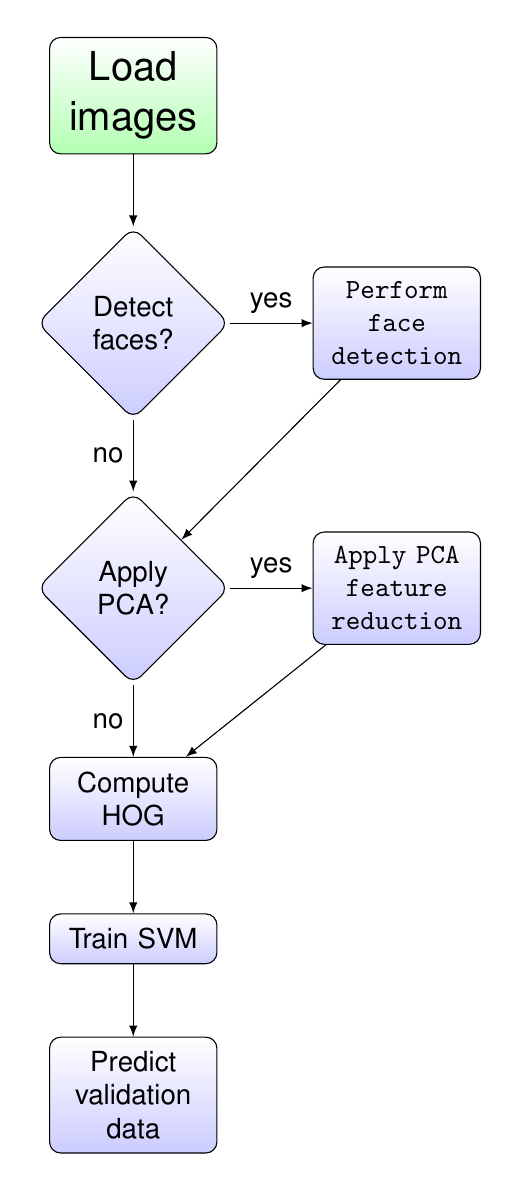
\begin{tikzpicture}[-latex][H]
  \matrix (chart)
    [
      matrix of nodes,
      column sep      = 3em,
      row sep         = 5ex,
      column 1/.style = {nodes={decision}},
      column 2/.style = {nodes={env}}
    ]
    {
      |[root]| Load images           &                \\
      Detect faces?               & Perform face detection       \\
      Apply PCA?                 & Apply PCA feature reduction         \\
     |[treenode]| Compute HOG  & \\
     |[treenode]| Train SVM &        \\
      |[treenode]| Predict validation data  &        \\
    %   & & |[decision]| numbered? \\
    %   & & |[treenode]| Add a \texttt{*} & |[finish]| Done \\
    };
    
  \draw
    (chart-1-1) edge (chart-2-1)
    \foreach \x/\y in {2/3, 3/4} {
      (chart-\x-1) \no (chart-\y-1) 
     }
    \foreach \x in {2,...,3} {
      (chart-\x-1) \yes (chart-\x-2)
    }
    (chart-2-2) edge (chart-3-1)
    (chart-3-2) edge (chart-4-1)
    
    (chart-4-1) edge (chart-5-1)
    (chart-5-1) edge (chart-6-1)
    ;

\end{tikzpicture}
\\
\\
The data module provides data types and data structures for the application. The class DataSet is the basic data type. It holds the images each together with the file name and the feature vectors extracted from that image. In the course of the main processing pipeline, the images themselves are deleted after the feature extraction step to free memory. The class furthermore provides a method to split the images and respectively their feature vectors into two parts of definable size for training and validation purpose. The class TrainingData holds the training and label matrix needed by the SVM for training in OpenCV matrix format. The constructor creates these matrices from the given vectors of positive and negative training samples, i.e. feature vectors.
\\
\\
The module IOUtils provides static methods for file system handling, input and output of images and basic image operations. There are methods to load a complete cataloge of images and methods to load single images or all images contained in a folder. In a cataloge of images, the images have to be organized in sub folders according to their categories and the sub folder names define the category names. There are methods to load and save SVMs from and to the file system. Furthermore, basic image operations like histogram equalization and adding flipped versions of images are part of this module as this functionality is integrated into the loading process to avoid memory issues due to allocation of images multiple times during the according process.
\\
TODO this structure needs to be changed in code, move stuff to utils!
\\
\\
The featureExtraction module provides the functionality for the HOG feature extraction. The class umHOG provides static methods to compute the HOG features for a DataSet object or a single image in OpenCV matrix format. It makes use of the OpenCV HOGDescriptor class to accomplish this task. The feature vectors are of the type vector of floats. The parameters for the extraction process correspond to those needed for the OpenCV HOGDescriptor extraction method. Furthermore the class provides a method to visualize the extracted gradients together with the original image. This method  has been enhanced to support generic input sizes and print out concrete values for gradient average or distinct gradients per extracted cell. The class umPCA provides static methods to reduce the dimensionality of the feature space. It makes use of the OpenCV PCA class and applies the Principal Component Analysis on the cells of the HOG features reducing the dimensionality to the number of gradient bins per cell.
%\footnote{http://www.juergenwiki.de/work/wiki/doku.php?id\=public:hog\_descriptor\_computation\_and\_visualization\#computing\_the\_hog\_descriptor\_using\_opencv}
\\
\\
The svm module provides the functionality for the machine learning parts of the processing pipeline. The class umSVM holds an object of OpenCV CvSVM and provides methods to train this SVM instance, to predict data and load and save this instance. The SVM instance is of type linear SVM C\_SVC, which can be configured using the SVM C value to refine the hyperplane on imperfect separation. The class ClassificationSVM holds a map of categorized umSVM instances and provides necessary methods to interact with them. These methods include training the SVMs on the complete cataloge of images, loading and saving categorized SVMs, and using the SVM instances for prediction.
\\
\\
TODO needs to be moved in code !!
\\
The class CatalogeTraining defines the main processing pipeline for training categorized SVMs with a cataloge of categorized images. The processing pipeline for single patch images, i.e. manual extracted patches, is setup like this:

\begin{enumerate}
	\item Loading an image cataloge from disc.
	\item Refine the images through histogram equalization.
	\item Double the sample size by adding flipped versions (Optional).
	\item Compute the HOG features for the images.
	\item Setup training and validation data.
	\item Train the SVMs on the training data.
	\item Validate the SVMs through prediction of the validation data.
	\item Exchange training and validation data and retrain the SVMs (Optional).
\end{enumerate}

In the course of the process, according methods of the application modules are invoked. The class itself handles the data setup. The class holds a map of categorized DataSets and maps for categorized TrainingData for training and validation purpose. It provides methods to collect positive and negative training samples, from which the TrainingData instances are constructed. These methods ensure equality of the size of positive and negative samples and an even distribution of negative samples among all other categories apart from the current positive one as far as the category sizes permit such equality and even distribution.
\\
\\
The class Configuration holds the configurable parameters for the application. The parameters are loaded from a given configuration file on instance construction. The class Constants holds the application parameters, that are not supposed to change during normal usage. This includes standard values for the SVM labels and debug flags for debugging the application.

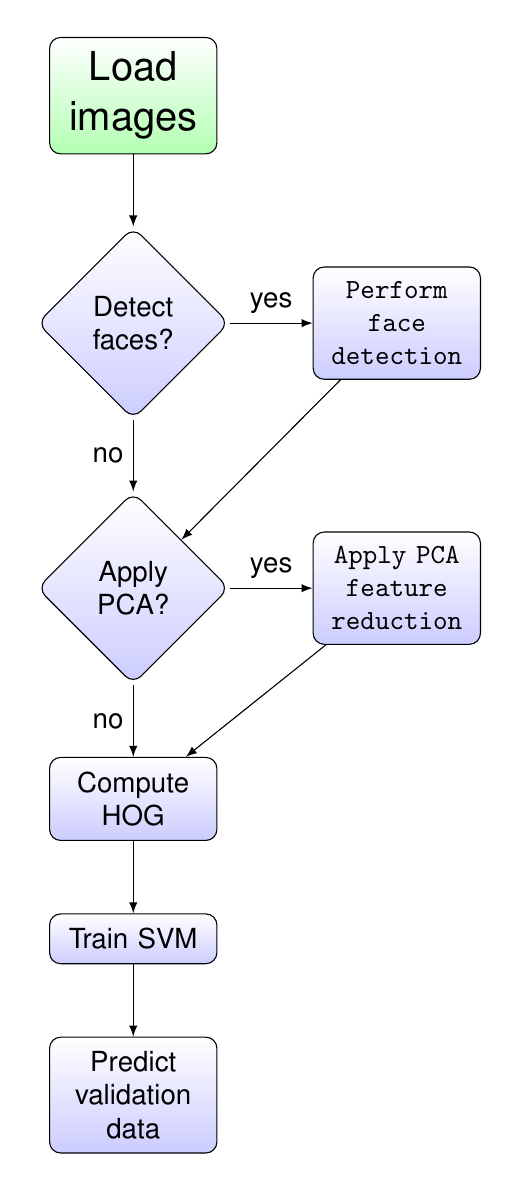
\begin{tikzpicture}[-latex][H]
  \matrix (chart)
    [
      matrix of nodes,
      column sep      = 3em,
      row sep         = 5ex,
      column 1/.style = {nodes={decision}},
      column 2/.style = {nodes={env}}
    ]
    {
      |[root]| Load images           &                \\
      Detect faces?               & Perform face detection       \\
      Apply PCA?                 & Apply PCA feature reduction         \\
     |[treenode]| Compute HOG  & \\
     |[treenode]| Train SVM &        \\
      |[treenode]| Predict validation data  &        \\
    %   & & |[decision]| numbered? \\
    %   & & |[treenode]| Add a \texttt{*} & |[finish]| Done \\
    };
    
  \draw
    (chart-1-1) edge (chart-2-1)
    \foreach \x/\y in {2/3, 3/4} {
      (chart-\x-1) \no (chart-\y-1) 
     }
    \foreach \x in {2,...,3} {
      (chart-\x-1) \yes (chart-\x-2)
    }
    (chart-2-2) edge (chart-3-1)
    (chart-3-2) edge (chart-4-1)
    
    (chart-4-1) edge (chart-5-1)
    (chart-5-1) edge (chart-6-1)
    ;

\end{tikzpicture}

% Bibliography:
%\clearpage
\addcontentsline{toc}{section}{Bibliography}

%\end{multicols}

\bibliographystyle{apalike}
\bibliography{./tex/report}

%\section{Project Contributions}

\begin{itemize}
	\item Stefan Selzer
	\begin{itemize}
	\item Complete code development, except for kmeans and part of face detection
	\item Complete thinking, planning and organization
	\item 1/4 of first presentation
	\item Structure, experiments and results for second presentation
	\item Complete Structure, Abstract, Sections 1,2,3, part of 5, half of Section 7 and Appendices of final Report
	\item Additional data
	\end{itemize}
	\item Chang Sun
	\begin{itemize}
	\item Some small error corrections in the code, part of k-means and face detection.
	\item Data acquisition
	\item 1/4 of first presentation
	\item dataset part of second presentation
	\item Part of manual patch extraction for second period
	\item Manual patch extraction
	\item Experiments and results for final report
	\item Part of sections 4,5,6
	\end{itemize}
	\item Salil Baht
	\begin{itemize}
	\item 1/4 of first presentation
	\item Part of manual patch extraction for second period
	\item Manual patch extraction
	\item Part of sections 4,5,6,7
	\end{itemize}
	\item Ioannis Papadopoulos
	\begin{itemize}
	\item Some small error corrections in the code, part of k-means.
	\item 1/4 of first presentation
	\item Gaussian blur filtering to generate additional input images for second period (unfortunately missing in code), experiments on that
	\item layout of the second presentation
	\item Part of sections 5,6,7
	\end{itemize}
\end{itemize}


\end{document}
